\problemname{Signs}
\noindent
After hearing rumors about the mutated giant rats in Gothenburg's sewers, your closest friends decided to flee up to the wonderful Stockholm. 
During their escape, your friends noticed that strangely there were a lot of road signs along the way to Stockholm pointing 
to various small villages near Lund. Additionally, the numbers on the signs seemed suspicious, as some of the signs contradicted the information on other signs.

On each of the $N$ road signs that your friends passed by, there are distances to all $M$ villages in Lund. 
The distances are rounded to the nearest integer, as the actual distance may not necessarily be an integer. 
Since your good friends happen to have a perfect photographic memory, they remember exactly which distances were stated on the signs. 
However, your friends do not remember when or in what order they saw these $N$ signs.

You can assume that Stockholm, Gothenburg, and the small villages in Lund all lie on a single straight line. 
Additionally, you can assume that all cities, villages, and signs are so small that they can be represented as 
points on this line. You can also assume that none of Lund's villages are located between two signs. 
In other words, the villages in Lund and the direction signs are on opposite sides of Gothenburg. 
Neither the villages nor the signs need to be placed at integer positions.

\begin{centering}
  \begin{figure}[h]
      \centering
      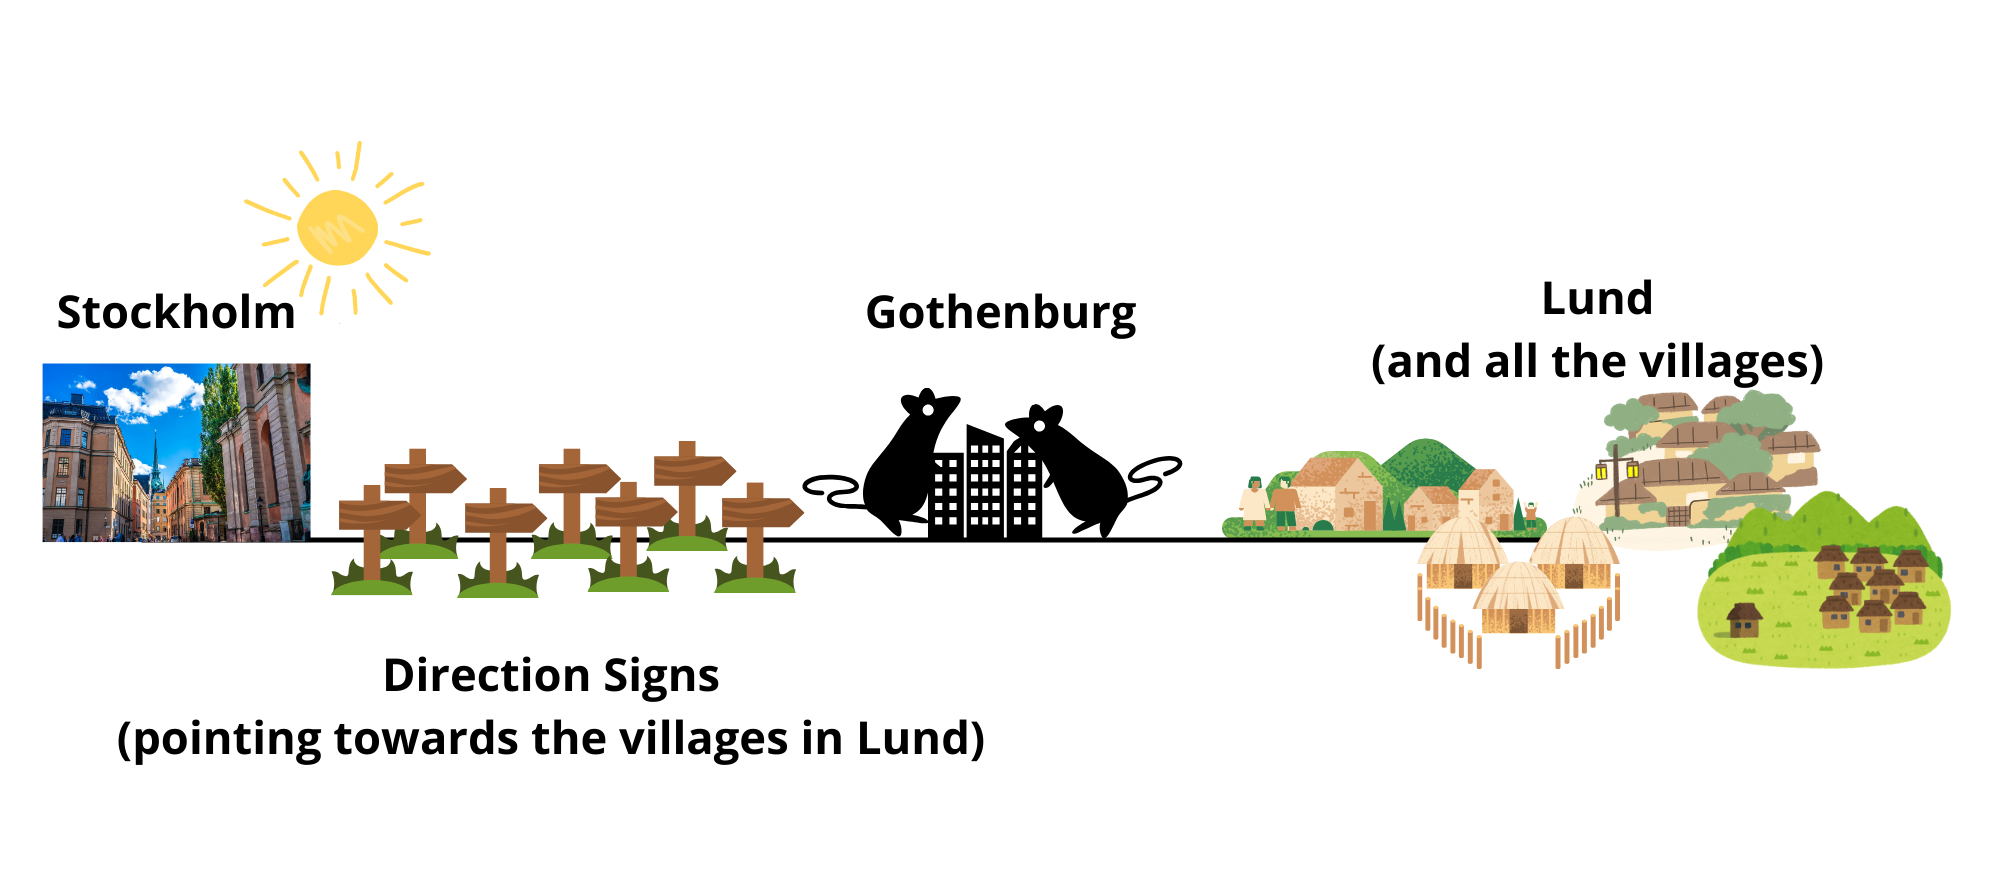
\includegraphics[width=0.8\textwidth]{skyltar.png}
      \caption{The illustration shows how the villages in Lund and the direction signs are on different sides of Gothenburg.}
  \end{figure}
\end{centering}

Given these $N$ signs that your friends have seen, what is the largest number of signs such that the distances given on the signs do not create any contradictions? 
Finally, you can also assume that at least $20\%$ of all signs are entirely correct and do not create any contradictions.


\section*{Input}
\noindent
The first line contains two integers $N$ and $M$ ($1 \leq N \leq 1000$, $1 \leq M \leq 200$), 
representing the number of signs your friends have seen and the number of villages in Lund, respectively.

The following $N$ lines of input each contain $M$ integers. The $i$-th line contains the integers $d_{i,1}, d_{i,2}, \ldots, d_{i,M}$ ($1 \leq d_{i,j} \leq 10^6$) describing the $M$ distances written on the $i$-th sign. 
So, on the $i$-th sign, it indicates that the distance from sign $i$ to village $j$ rounded down is $d_{i,j}$ for all $1 \leq j \leq M$.

\section*{Output}
\noindent
First, output on a single line an integer $t$, the maximum number of consistent signs.
On the second line, output $t$ integers specifying the indices in sorted order such that the first sign is the farthest from Gothenburg and all villages in Lund, 
and the last sign is the closest to Gothenburg and the all villages in Lund.
Since people in the society get confused when things are $0$-indexed, we want the signs to be $1$-indexed. 
So, the first sign in the input is indexed as $1$, and the last sign with index $N$.
If there are multiple valid solutions, your program can output any of these possible solutions.

\section*{Scoring}
Your solution will be tested on a set of test groups, each worth a number of points. 
Each test group contains a set of test cases. 
To get the points for a test group you need to solve all test cases in the test group.

\noindent
\begin{tabular}{| l | l | p{12cm} |}
  \hline
  \textbf{Group} & \textbf{Point value} & \textbf{Constraints} \\ \hline
  $1$    & $21$         & $N \leq 15, M \leq 50$.  \\ \hline
  $2$    & $31$         & $N \leq 100, M \leq 50$ \\ \hline
  $3$    & $18$         & $N \leq 500, M \leq 50$ \\ \hline
  $4$    & $30$         & No additional constraints. \\ \hline
\end{tabular}



\section*{Explanation of sample 1:}
Imagine a number line on the $x$-axis.
The second sign can be placed at position $x = 1$, 
and the first sign at position $x = 1\frac{1}{2}$, 
the first village at position $x = 3\frac{1}{2}$, 
and the second village at $x = 4$.

It's also possible to find a construction with signs number 1 and 3.

It's clear that signs 1 and 2 contradict each other, which means that there's no construction where all 3 signs are used.

\section*{Comment on sample 2:}
Note that all signs round down the distance to different numbers, even though all signs point to the same village.

\section*{Comment on sample 3:}
Note that all pairs of signs lead to a contradiction; any arbitrary sign would be a correct answer in this case.